\subsection{Stream Testing}
To address \textbf{RQ1} and \textbf{RQ3} we assigned two groups the task to model a Controller for PacMan and SuperMario respectively and interview the results afterwards. In the future we will refer to the groups as \textit{group A} and \textit{group B}. Group A consists of one subject who is familiar with EmbeddedMontiArc and group B consists of two subjects who have no experience with EmbeddedMontiArc. These groups were selected random among the students of a computer science seminar. 
EmbeddedMontiArc comes along with stream tests in order to check a component against a condition as stated in the previous chapter.
We can use those tests to define the conditions the controllers need to fulfill. Those conditions are taken from use cases. For PacMan the most general acceptance test would be to never let the PacMan die. Due to the fact that stream tests cannot be defined unlimited and that this test might be hard to implement we defined the following deterministic tests for PacMan and SuperMario. We first state those for PacMan:

\subsubsection{PacMan}
\begin{itemize}
	\item Given the scenario in fig. \ref{fig:pacmanLeft}, the PacMan must be controlled to the left (in order to not die)
	\item Given the scenario in fig. \ref{fig:pacmanEatable}, the PacMan should be controlled toward the blue ghost, sending him away from his current position.
	\item Given the scenario in fig. \ref{fig:pacmanCookie} (Zwei Wege sind gleichwertig, einer hat einen Cookie drin) the PacMan should navigate to the cookie.
\end{itemize}

\begin{figure}[!h]
	\centering
	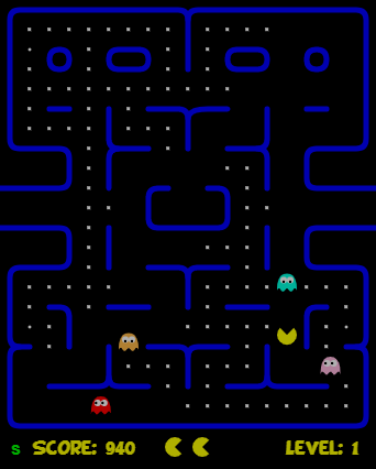
\includegraphics[scale=0.55]{pictures/Pacman_Condition3.PNG}
	\caption{PacMan has to go left in order to live}
	\label{fig:pacmanLeft}
\end{figure}
\begin{figure}[!h]
	\centering
	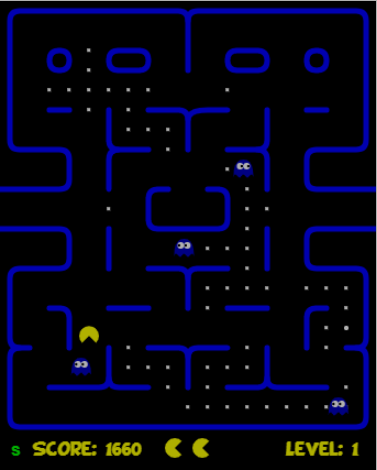
\includegraphics[scale=0.55]{pictures/Pacman_Condition4.PNG}
	\caption{Ghosts are eatable}
	\label{fig:pacmanEatable}
\end{figure}
\begin{figure}[!h]
	\centering
	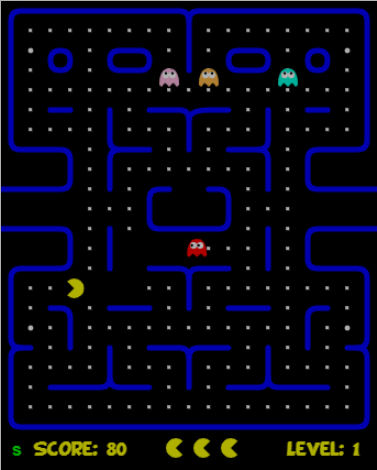
\includegraphics[scale=0.55]{pictures/Pacman_Condition6.PNG}
	\caption{Pacman can choose between going left or down}
	\label{fig:pacmanCookie}
\end{figure}

Those scenarios can be tested easily within a few ticks via stream testing.

\subsubsection{Supermario (by Philipp Haller)}


TESTING
The goal for the Supermario model is to solve a level successfully. The first level was chosen since it provides a diverse environment with different enemy types and obstacles, while not being too skill intensive to solve.  

In order to develop the model, different situations were assessed and according tests derived. The scenarios a SuperMario model has to master are listed in the following, while the derived tests are presented in chapter X.


DELETE MOST OF THIS!
\begin{itemize}
	\item Given the scenario in fig. \ref{fig:marioLeft}, Mario has to build up speed in order to jump over the obstacle.
	\item Given the scenario in fig. \ref{fig:marioSmashHead}, Mario has to jump in order to get coins, mushrooms or flowers.
	\item Given the scenario in fig. \ref{fig:marioEat}, Mario has to eat the mushroom in order to grow.
	\item Given the scenario in fig. \ref{fig:marioFight}, Mario has to jump on the evil mushrooms or evade them.
\end{itemize}

\begin{figure}[!h]
	\centering
	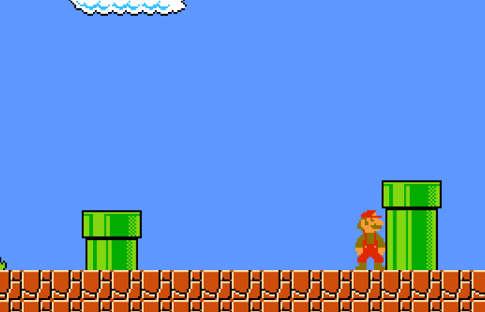
\includegraphics[scale=0.55]{pictures/Mario1.PNG}
	\caption{Mario has to go left in order jump over the obstacle}
	\label{fig:marioLeft}
\end{figure}
\begin{figure}[!h]
	\centering
	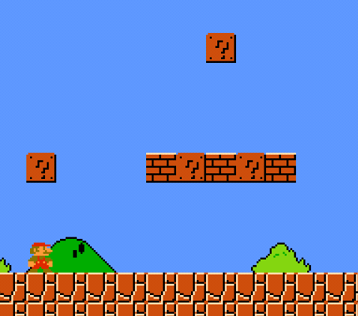
\includegraphics[scale=0.55]{pictures/Mario2.PNG}
	\caption{Mario with loot boxes over him}
	\label{fig:marioSmashHead}
\end{figure}
\begin{figure}[!h]
	\centering
	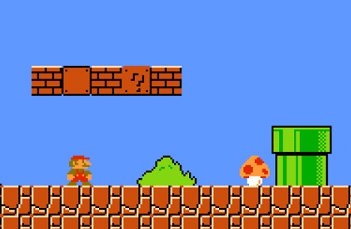
\includegraphics[scale=0.55]{pictures/Mario3.PNG}
	\caption{Mario with a mushroom}
	\label{fig:marioEat}
\end{figure}
\begin{figure}[!h]
	\centering
	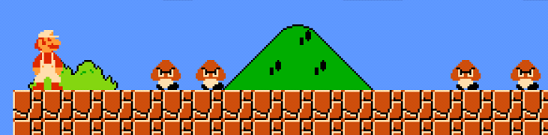
\includegraphics[scale=0.55]{pictures/Mario4.PNG}
	\caption{Mario with enemies}
	\label{fig:marioFight}
\end{figure}


VEREINFACHUNGEN?? WIESO? HIERHIN?
Prior to modeling some assumptions were made to fulfill time and complexity constraints.
Only a fixed number of enemies and obstacles in the path of the player are considered in order to ensure a static input size. Five entities each have shown empirically to be sufficient for the first level and the implemented strategy. For the same reason only the next hole in the ground is considered
-Why 5 enemies, obstacles etc
VEREINFACHUNGEN ENDE

Since the presented scenarios have in common that the player has to 

The two groups were then assigned to use these tests as a guideline to develop their controllers.

\subsection{Preparations (by Haller and Heithoff)}
The code of the Pacman emulator (Link?) and Supermario emulator \cite{marioLink} we used was available in Html5 and JavaScript. C\&C-Components in EmbeddedMontiArc can be translated to C++ code and then to a webassembly which uses JavaScript (see \cite{bertram2017component}). This JavaScript file can be given inputs according to the component and calculates the outputs on execution. To combine these two files, there is an additional interface needed to extract the information for the inputs out of the emulator and then give the calculated outputs into the emulator.
For the purpose of implementing the controllers the subjects were assigned to use EmbeddedMontiArcStudio.
EmbeddedMontiArcStudioV1.6.2 did neither support a simulator of PacMan nor of a simulator SuperMario. So an additional step to answer RQ2 \textit{Is it possible to integrate other simulators in a recent amount of work} it for the groups to integrate the simulators into the EmbeddedMontiArcStudio.
In order to be able to do so, group A is instructed by an expert (Jean-Marc) which files need modification and what to add. After that group A instructed group B the same way.

